% !TeX root = RJwrapper.tex
\title{did2s: Two-Stage Difference-in-Differences}
\author{by Kyle Butts and John Gardner}

\maketitle

\abstract{%
Recent work has highlighted the difficulties of estimating difference-in-differences models when the treatment is adopted at different times for different units. This article introduces the R package \CRANpkg{did2s} which implements the estimator introduced in Gardner (2022). The article provides an approachable review of the underlying econometric theory and introduces the syntax for the function \texttt{did2s}. Further, the package introduces functions, event\_study and plot\_event\_study, which uses a common syntax to implement all of the modern event-study estimators.
}

\hypertarget{introduction}{%
\subsection{Introduction}\label{introduction}}

A rapidly growing econometric literature has identified difficulties in traditional difference-in-differences estimation when treatment turns on at different times for different groups and when the effects of treatment vary across groups and over time (Callaway and Sant'Anna 2020; Sun and Abraham 2020; Goodman-Bacon 2018; Borusyak, Jaravel, and Spiess 2021; Chaisemartin and D'Haultfoeuille 2019). Gardner (2022) proposes an estimator of the two-way fixed-effects model that is quick and intuitive. The estimator relies on the standard two-way fixed-effect model (see the following section) and forms an intuitive estimate: the average difference in outcomes between treated and untreated units after removing fixed unit- and time-invariant shocks.

This article first discusses the modern difference-in-differences theory in an approachable way and second discusses the software package, \CRANpkg{did2s}, which implements the two-stage estimation approach proposed by Gardner (2022) to estimate robustly the two-way fixed-effects (TWFE) model. There are two notable technical features of this package. First, \texttt{did2s} utilizes the incredibly fast package, \CRANpkg{fixest} (Bergé 2018), which can estimate regressions with a high number of fixed-effects very quickly. Second, since there are a few alternative TWFE event-study estimators implemented in \texttt{R}, each with their own syntax and data formatting requirements, the package also has a set of functions that allow quick estimation and plotting of every alternative event study estimator using a standardized syntax. This allows for easy comparison between the results of different methods.

\hypertarget{difference-in-differences-theory}{%
\subsection{Difference-in-differences theory}\label{difference-in-differences-theory}}

Researchers commonly use the difference-in-differences (DiD) methodology to estimate the effects of treatment in the case where treatment is non-randomly assigned. Instead of random assignment giving rise to identification, the DiD method relies on the so-called ``parallel trends'' assumption, which asserts that outcomes would evolve in parallel between the treated and untreated groups \emph{in a world where the treated were untreated}. This is formalized with the \emph{two-way fixed-effects} (TWFE) model. In a static setting where treatment effects are \emph{constant} across treatment groups and over time, researchers estimate the \textbf{static TWFE model}:
\begin{equation}\label{eq:twfe}
  y_{igt} = \mu_g + \eta_t + \tau D_{gt} + \varepsilon_{igt},
\end{equation}
where \(y_{igt}\) is the outcome variable of interest, \(i\) denotes the individual, \(t\) denotes time, and \(g\) denotes group membership where a ``group'' is defined as all units that start treatment at time \(g\).\footnote{In the literature, never treated units often are given a value of \(g = \infty\).} \(\mu_g\) is a vector of time-invariant group fixed-effects, \(\eta_t\) is a vector of shocks in a given time period that is experienced by all individuals equally, and \(D_{gt}\) is an indicator for whether initial-treatment group \(g\) is receiving treatment in period \(t\), i.e.~\(D_{gt} \equiv \mathbb{1}(g \leq t)\). The coefficient of interest is \(\tau\), which is the \textbf{(\emph{constant}) average effect of the treatment on the treated} (ATT). If it is indeed true that the treatment effect is constant across groups and over time, then the estimate formed by estimating the static TWFE model will be consistent for \(\tau\) under a parallel trends assumption on the error term.

However, treatment effects are not constant in most settings. The magnitude of a unit's treatment effect can differ based on group status \(g\) (e.g.~if groups that benefit more from a policy implement it earlier) and treatment duration (e.g.~if treatment effects grow as the policy has been in place for longer periods). Therefore to enrich our model, we allow heterogeneity in treatment effects across \(g\) and \(t\) by introducing the \textbf{group-time average treatment effect}, \(\tau_{gt}\). Correspondingly, we modify the TWFE model as follows:
\[
  y_{igt} = \mu_g + \eta_t + \tau_{gt} D_{gt} + \varepsilon_{igt}.
\]
The key difference is that treatment effects are allowed to differ based on group status \(g\) and time period \(t\). Estimating any individual \(\tau_{gt}\) may not be desirable since there would be too few observations. Instead, researchers aggregate group-time average treatment effects into the \textbf{overall average treatment effect}, \(\tau\), which averages across \(\tau_{gt}\):
\[
  \tau \equiv \sum_{g, t} \frac{N_{gt}}{N_{post}} \tau_{gt},
\]
where \(N_{gt}\) denotes the number of observations in \((g, t)\) and \(N_{post}\) is the number of post-treatment observations (\(t \geq g\)). The natural question is, ``does the static TWFE model, (\ref{eq:twfe}), produce a consistent estimate for the overall average treatment effect?'' Except for a few specific scenarios, the answer is no (Sun and Abraham 2020; Goodman-Bacon 2018; Borusyak, Jaravel, and Spiess 2021; Chaisemartin and D'Haultfoeuille 2019).

One way of thinking about this disappointing result is through the Frisch--Waugh--Lovell (FWL) theorem (Frisch and Waugh 1933). This theorem says that estimating the Static TWFE model is equivalent to estimating
\[
y_{igt} - \hat{\mu}_g - \hat{\eta}_t = \tau \tilde{D}_{gt} + \tilde{\varepsilon}_{gt},
\]
where \(\tilde{D}_{gt}\) denotes the residuals from regressing \(D_{gt}\) on \(\mu_g\) and \(\eta_t\); \(\hat{\mu}_g\) and \(\hat{\eta}_t\) are estimates for the group and time fixed-effects, respectively. The left-hand side of this equation, under a parallel trends restriction on the error term \(\varepsilon_{it}\), is our estimate for \(\tau_{gt}\). Therefore, the FWL theorem tells us estimating the static TWFE model is equivalent to estimating\footnote{This is a minor abuse of notation since \(y_{igt} - \hat{\mu}_g - \hat{\eta}_t\) is an estimate for \(\tau_{igt}\) which can be different from \(\tau_{gt}\) if there is within group-time heterogeneity.}

\[
\hat{\tau}_{gt} = \tau \tilde{D}_{gt} + \tilde{\varepsilon}_{gt}
\]

The resulting estimate for \(\tau\) can be written as:
\[
\hat{\tau} \equiv \sum_{g,t} w_{gt} \hat{\tau}_{gt},
\]
where \(w_{gt}\) is the weight put on the corresponding \(\hat{\tau}_{gt}\). Results of Gardner (2022), Borusyak, Jaravel, and Spiess (2021), and Chaisemartin and D'Haultfoeuille (2019) all characterize the weights \(w_{gt}\) from this regression. There are only two cases where the \(\hat{\tau}\) is a consistent estimate for the overall average treatment effect. First, when treatment occurs at the \emph{same time} for all treated units, then \(w_{gt}\) is equal to \(N_{gt}/N_{post}\) for all \(\{g, t\}\) and therefore \(\hat{\tau}\) is a consistent estimate for the overall average treatment effect. The other scenario where \(\hat{\tau}\) estimates the overall average treatment effect is when \(\tau_{gt}\) is constant across group and time, i.e.~\(\tau_{gt} = \tau\). Since the weights, \(w_{gt}\), always sum to one, we have that \(\hat{\tau} = \sum w_{gt} \hat{\tau}_{gt} \to \sum w_{gt} \tau = \tau\).

The above cases are not the norm in research. If there is heterogeneity in group-time treatment effects \emph{and} units get treated at different times, then \(\hat{\tau}\) is not a consistent estimate for the average treatment effect \(\tau\). Instead, \(\hat{\tau}\) will be a weighted average of group-time treatment effects with some weights, \(w_{gt}\), being potentially negative. This yields a treatment effect estimate that does not provide a good summary of the ``average'' treatment effect. It is even possible for the sign of \(\hat{\tau}\) to differ from that of the overall average treatment effect. This would occur, for example, if negative weights are placed primarily on the largest (in magnitude) group-time treatment effects.

To summarize the modern literature, the fundamental problem faced in estimating the TWFE model is the potential negative weighting. The proposed methodology in Gardner (2022) is based on the fact that if \(\hat{\tau}_{gt}\) is regressed on \(D_{gt}\), instead of \(\tilde{D}_{gt}\), the resulting weights would be exactly equal to \(N_{gt}/N_{post}\) and the coefficient of \(D_{gt}\) would estimate the overall average treatment effect.

\hypertarget{event-study-estimates}{%
\subsubsection{Event-study estimates}\label{event-study-estimates}}

Researchers have attempted to model treatment effect heterogeneity by allowing treatment effects to change over time. To do this, they introduce a (dynamic) event-study TWFE model:
\begin{equation}
  y_{igt} = \mu_g + \eta_t + \sum_{k = -L}^{-2} \tau^k D_{gt}^k + \sum_{k = 0}^{K} \tau^k D_{gt}^k + \varepsilon_{igt},
\end{equation}
where \(D_{gt}^k\) are lags/leads of treatment (\(k\) periods from initial treatment date). The coefficients of interests are the \(\tau^k\), which represent the average effect of being treated for \(k\) periods. For negative values of \(k\), \(\tau^k\) are known as ``pre-trends,'' and represent the average deviation in outcomes for treated units \(k\) periods away from treatment, relative to their value in the reference period. These pre-trend estimates are commonly used as a test of the parallel counterfactual trends assumption.

Our goal is to estimate the \textbf{average treatment effect of being exposed for \(k\) periods}, an average of \(\tau_{gt}\) for only the set of \(\{g,t\}\) where \(k\) periods have elapsed since \(g\), i.e.~\(t - g = k\):
\[
  \tau^k = \sum_{g,t \ : \ t - g = k} \frac{N_{gt}^k}{N^k} \tau_{gt},
\]
where the sum is over \(\{g,t\}\) with \(t - g = k\), \(N_{gt}^k\) is the number of observations in group \(g\) and \(N^k\) is the total number of observations with \(t - g = k\). The results of Sun and Abraham (2020) show that even though we allow for our average treatment effects to vary over time \(\tau^k\), the negative weighting problems would arise if units are treated at different times \emph{and} there is group-heterogeneity in treatment effects. Similar to the static TWFE model, the estimates of \(\tau^k\) from running the event-study model form non-intuitively weighted averages of \(\tau_{gt}\) with \(w_{gt}^k \neq N_{gt}^k/N^k\). Even worse, the group-time treatment effects for \(t-g \neq k\) will be included in the estimate of \(\hat{\tau}^k\). Hence, the need for a robust difference-in-differences estimator remains even in the event-study model.

\hypertarget{two-stage-difference-in-differences-estimator}{%
\subsubsection{Two-stage difference-in-differences estimator}\label{two-stage-difference-in-differences-estimator}}

Gardner (2022) proposes an estimator to resolve the problem with the two-way fixed-effects approaches. Rather than attempting to estimate the group and time effects simultaneously with the ATT (causing \(D_{it}\) to be residualized), Gardner's approach proceeds from the observation that, under parallel trends, the group and time effects are identified from the subsample of untreated/not-yet-treated observations (\(D_{gt} = 0\)). This suggests a simple two-stage difference-in-differences estimator:

\begin{enumerate}
\def\labelenumi{\arabic{enumi}.}
\item
  Estimate the model
  \[
   y_{igt} = \mu_g + \eta_t + \varepsilon_{igt},
  \]
  using the subsample of untreated/not-yet-treated observations (i.e., all observations for which \(D_{gt}=0\)), retaining the estimated group and time effects to form the adjusted outcomes \(\tilde{y}_{igt} \equiv y_{igt} - \hat{\mu}_g - \hat{\eta}_t\).
\item
  Regress adjusted outcomes \(\tilde{y}_{igt}\) on treatment status \(D_{gt}\) or \(D_{gt}^k\) in the full sample to estimate treatment effects \(\tau\) or \(\tau^k\).
\end{enumerate}

To see why this procedure works, note that parallel trends implies that outcomes can be expressed as
\begin{align*}
  y_{igt} &= \mu_g + \eta_t + \tau_{gt} D_{gt} + \varepsilon_{igt} \\
  &= \mu_g + \eta_t + \bar{\tau} D_{gt} + (\tau_{gt} - \bar{\tau}) D_{gt} + \varepsilon_{igt},
\end{align*}
where \(\tau_{gt} = E(Y^1_{igt} - Y^0_{igt} \ | \ g, t)\) is the average treatment effect for group \(g\) in period \(t\)\footnote{i.e., the average difference between treated and untreated potential outcomes \(y^1_{igt}\) and \(y^0_{igt}\), conditional on the observed treatment-adoption times.} and \(\bar{\tau} = E(\tau_{gt} | D_{gt}=1)\) is the overall average treatment effect\footnote{i.e., the population-weighted average of the group-time specific ATTs, \(\tau_{gt}\).}. Note from parallel trends, \(E(\varepsilon_{igt} | D_{gt}, g, t) = 0\). Rearranging, this gives
\[
  y_{igt} - \mu_g - \eta_t = \bar{\tau} D_{gt} + (\tau_{gt} - \bar{\tau}) D_{gt} + \varepsilon_{igt}.
\]
Suppose you knew the time and group fixed-effects and were able to directly observe the left-hand side (later we will estimate the left-hand side). Regressing the adjusted \(y\) variable, on \(D_{gt}\) will produce a consistent estimator for \(\bar{\tau}\). To see this, note that \(E[(\tau_{gt} - \bar{\tau}) D_{gt} \ | \ D_{gt}] = 0\). Hence, the treatment dummy is uncorrelated with the omitted variable and the average treatment effect is identified in the second-stage. Since we are not able to directly observe \(\mu_g\) and \(\eta_t\), we estimate them using the untreated/not-yet-treated observations in the first-stage. However, standard errors need adjustment to account for the added uncertainty from the first-stage estimation.

This approach can be extended to dynamic models by replacing the second stage of the procedure with a regression of residualized outcomes onto the leads and lags of treatment status, \(D_{gt}^k\), \(k \in \{-L, \dots, K\}\). Under parallel trends, the second-stage coefficients on the lags identify the overall average effect of being treated for \(k\) periods (where the average is taken over all units treated for at least that many periods). The second-stage coefficients on the leads identify the average deviation from predicted counterfactual trends among units that are \(k\) periods away from treatment, which under parallel trends should be zero for any pre-treatment value of \(k\). Hence, the coefficients on the leads represent a test of the validity of the parallel trends assumption.

\hypertarget{inference}{%
\subsubsection{Inference}\label{inference}}

The standard variance-covariance matrix from the second-stage regression will be incorrect since it fails to account for the fact that the dependent variable is generated from the first-stage regression. However, this estimator takes the form of a joint generalized method of moments (GMM) estimator whose asymptotic variance is well understood (Newey and McFadden 1986).

Specifically, the estimator takes the form of a two-stage GMM estimator with the following two moment conditions:
\begin{align}
  m(\theta) = (Y-X_{10}'\gamma)X_{10}, \\
  g(\gamma, \theta) = (Y - X_1'\gamma - X_2'\theta) X_2,
\end{align}
where \(X_1\) is the matrix of group and time fixed-effects, \(X_{10}\) corresponds to the matrix \(X_1\), but with rows corresponding to observations for which \(D_{gt} = 1\) replaced with zeros (as only observations with \(D_{gt} = 0\) are used in the first stage) and \(X_2\) is the matrix of treatment variable(s). The first equation corresponds with the first stage and the second equation corresponds with the second stage. From Theorem 6.1 of Newey and McFadden (1986), the asymptotic variance of the two-stage estimator is
\begin{equation}
  V = G_\theta^{-1} E\left[ (g + G_\gamma \psi)(g + G_\gamma \psi)' \right] G_\theta^{-1'},
\end{equation}
where from our moment conditions, we have:
\[
  G_\theta = - E\left(X_2X_2' \right),
\]
\[
  G_\gamma = - E\left(X_2X_1'\right),
\]
\[
  \psi = E(X_{10}X_{10}')^{-1} \varepsilon_{10} X_{10}.
\]

This can be estimated using
\begin{equation}
  \left(X_2'X_2\right)^{-1} \left(\sum_{g=1}^G W_g' W_g\right) \left(X_2'X_2\right)^{-1},
\end{equation} where
\[
  W_g = X_{2g}'\hat{\varepsilon}_{2g} - \hat{\varepsilon}_{10g}' X_{1g}\left(X_{1g}'X_{1g}\right)^{-1} \left(X_{1g}'X_{2g}\right),
\]
and matrices indexed by \(g\) correspond to the \(g\)th cluster.

\hypertarget{the-package}{%
\subsection{\texorpdfstring{The \CRANpkg{did2s} package}{The  package}}\label{the-package}}

The \CRANpkg{did2s} package introduces two sets of functions. The first is the \texttt{did2s} command which implements the two-stage difference-in-differences estimator as described above. The second is the \texttt{event\_study} and \texttt{plot\_event\_study} commands that allow individuals to implement alternative `robust' estimators using a singular common syntax.

\hypertarget{the-did2s-command}{%
\subsubsection{\texorpdfstring{The \texttt{did2s} command}{The did2s command}}\label{the-did2s-command}}

The command \texttt{did2s} implements the two-stage difference-in-differences estimator following Gardner (2022). The general syntax is

\begin{verbatim}
did2s(data, yname, first_stage, second_stage, 
      treatment, cluster_var, weights = NULL, 
      bootstrap = FALSE, n_bootstraps = 250, 
      verbose = TRUE)
\end{verbatim}

and full details on the arguments is available in the help page, available by running \texttt{?did2s}. There are a few arguments that are worth discussing in more detail.

The \texttt{first\_stage} and \texttt{second\_stage} arguments require formula arguments. These formulas are passed to the \texttt{fixest::feols} function from \CRANpkg{fixest} and can therefore utilize two non-standard formula options that are worth mentioning (Bergé 2018). First, fixed-effects can be inserted after the covariates, e.g.~\texttt{\textasciitilde{}\ x1\ \textbar{}\ fe\_1\ +\ fe\_2}, which will make estimation much faster than using \texttt{factor(fe\_1)}. Second, the function \texttt{fixest::i} can be used for treatment indicators instead of \texttt{factor}. The advantage of this is that you can easily specify the reference values, e.g.~for event-study indicators where researchers typically want to drop time \(t = -1\), \texttt{\textasciitilde{}\ i(rel\_year,\ ref\ =\ c(-1))} would be the correct second-stage formula. Additionally, \CRANpkg{fixest} has a number of post-estimation exporting commands to make tables with \texttt{fixest::etable} and event-study plots with \texttt{fixest::iplot}/\texttt{fixest::coefplot}. The \texttt{fixest::i} function is better integrated with these functions as we will see below.

The option \texttt{treatment} is the variable name of a \(0/1\) variable that denotes when treatment is active for a given unit, \(D_{gt}\) in the above notation. Observations with \(D_{gt} = 0\) will be used to estimate the first stage, which removes the problem of treatment effects contaminating estimation of the unit and time fixed-effects. However, as an important note, if you suspect anticipation effects before treatment begins, the \texttt{treatment} variable should be shifted forward by \(x\) periods for observations to prevent the aforementioned contamination. For example, if you suspect that units could experience treatment effects 1 period ahead of treatment (a so-called anticipatory effect), then the \texttt{treatment} should begin one period ahead. These anticipation effects can be estimated, after adjusting the \texttt{treatment} variable, by using a reference year of say, \(t = -2\) and looking at the estimate for relative year \(-1\).

\hypertarget{example-usage-of-did2s}{%
\paragraph{\texorpdfstring{Example usage of \texttt{did2s}}{Example usage of did2s}}\label{example-usage-of-did2s}}

For basic usage, I will use the simulated dataset, \texttt{df\_het}, that comes with the \CRANpkg{did2s} package with the command

\begin{verbatim}
data(df_het, package = "did2s")
\end{verbatim}

The data-generating process is displayed in Figure \ref{fig:ex-data}. The lines represent the mean outcome for each treatment group and the never-treated group. In the absence of treatment, each group is simulated to be on parallel trends. There is heterogeneity in treatment effects both within a treatment group over time and across treatment groups.

\begin{figure}
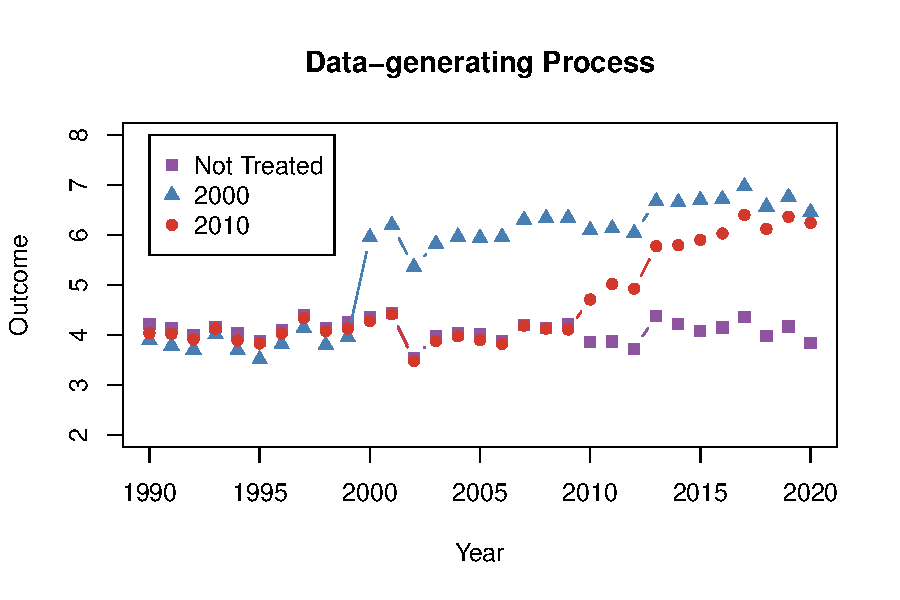
\includegraphics[width=1\linewidth]{RJ-2022-048_files/figure-latex/ex-data-1} \caption{This figure plots simulated data with two treated groups and a never-treated group. Each line represents the average outcome (y-value) in a given year (x-value) for each of the three groups. In the absence of treatment, all three groups would exhibit parallel trends (staying around a value of 4 in each period). Each of the treated groups are experience different treatment effect magnitudes that grow over time. This treatment effect heterogeneity creates problems for the classical two-way fixed effect OLS estimator.}\label{fig:ex-data}
\end{figure}

First, we will calculate a static difference-in-differences estimate using the \texttt{did2s} function.

\begin{verbatim}
static = did2s(
    data = df_het, 
    yname = "dep_var", 
    treatment = "treat",
    first_stage = ~ 0 | unit + year, 
    second_stage = ~ i(treat, ref = FALSE),
    cluster_var = "unit", 
    verbose = FALSE
)

summary(static)
\end{verbatim}

\begin{verbatim}
#> OLS estimation, Dep. Var.: dep_var
#> Observations: 46,500 
#> Standard-errors: Custom 
#>             Estimate Std. Error t value  Pr(>|t|)    
#> treat::TRUE  2.23048   0.021408  104.19 < 2.2e-16 ***
#> ---
#> Signif. codes:  0 '***' 0.001 '**' 0.01 '*' 0.05 '.' 0.1 ' ' 1
#> RMSE: 1.0357   Adj. R2: 0.505683
\end{verbatim}

Since the returning object is a \texttt{fixest} object, all the accompanying output commands from \CRANpkg{fixest} are available to use. For example, we can create regression tables:

\begin{verbatim}
fixest::etable(static, fitstat = c("n"), tex = TRUE,
  title = "Estimate of Static TWFE Model", 
  notes = "This table presents the estimated overall treatment effect. The effect is estimated using Two-Stage Difference-in-Differences proposed by Gardner (2021). The estimated effect is close to the true value.")
\end{verbatim}

\begin{table}[htbp]
   \caption{Estimate of Static TWFE Model}
   \centering
   \begin{tabular}{lc}
      \tabularnewline \midrule \midrule
      Dependent Variable: & dep\_var\\   
      Model:              & (1)\\  
      \midrule
      \emph{Variables}\\
      treat $=$ TRUE      & 2.230$^{***}$\\   
                          & (0.0214)\\   
      \midrule
      \emph{Fit statistics}\\
      Observations        & 46,500\\  
      \midrule \midrule
      \multicolumn{2}{l}{\emph{Custom standard-errors in parentheses}}\\
      \multicolumn{2}{l}{\emph{Signif. Codes: ***: 0.01, **: 0.05, *: 0.1}}\\
   \end{tabular}
   
   \par \raggedright 
   This table presents the estimated overall treatment effect. The effect is estimated using Two-Stage Difference-in-Differences proposed by Gardner (2021). The estimated effect is close to the true value.
\end{table}

However, since there are dynamic treatment effects in this example, it is much better to estimate the dynamic effects themselves using an event-study specification. We will then plot the results using \texttt{fixest::iplot}, which plots coefficients corresponding to an \texttt{i()} variable. Note that \texttt{rel\_year} is coded as \texttt{Inf} for never-treated units, so this has to be noted in the reference part of the formula.

\begin{verbatim}
es = did2s(
    data = df_het, 
    yname = "dep_var", 
    treatment = "treat",
    first_stage = ~ 0 | unit + year, 
    second_stage = ~ i(rel_year, ref = c(-1, Inf)),
    cluster_var = "unit", 
    verbose = FALSE
)

fixest::iplot(
    es, 
    main = "Event study: Staggered treatment", 
    xlab = "Relative time to treatment", 
    col = "steelblue", ref.line = -0.5
)

# Add the (mean) true effects
true_effects = tapply((df_het$te + df_het$te_dynamic), df_het$rel_year, mean)
true_effects = head(true_effects, -1)
points(-20:20, true_effects, pch = 20, col = "grey60")

# Legend
legend(x=-20, y=3, col = c("steelblue", "grey60"), 
       pch = c(20, 20), 
       legend = c("Two-stage estimate", "True effect"))
\end{verbatim}

\begin{figure}
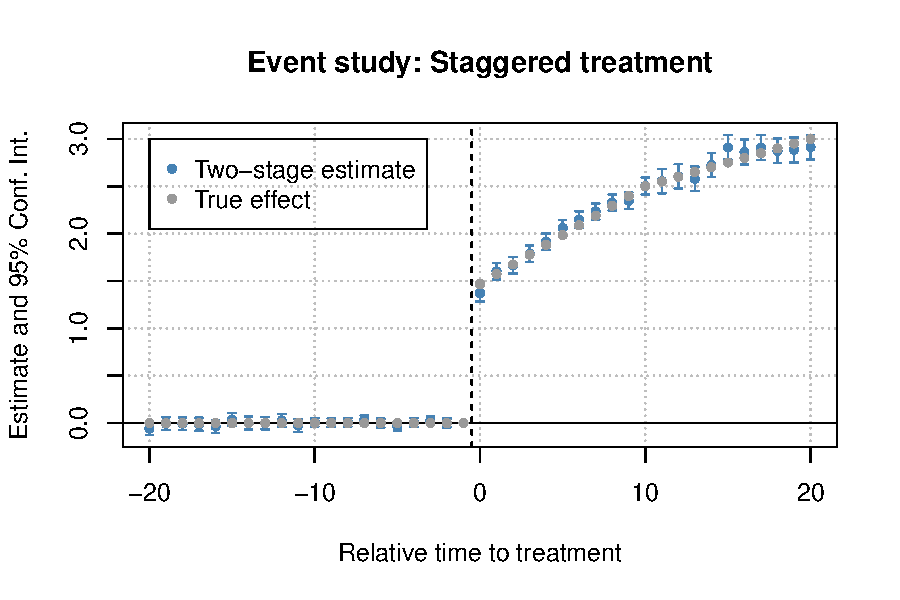
\includegraphics[width=1\linewidth]{RJ-2022-048_files/figure-latex/dynamic-1} \caption{This figure plots the true treatment effect and estimates using the Two-Stage Difference-in-Differences proposed by Gardner (2021). The x-axis of this figure is the relative time to treatment, i.e. how many years pre-/post- treatment that period is. The y-axis is estimated treatment effects. There are two sets of points. The first is for the true effect which is equal to 0 in all pre-periods and in the post-period starts at 1.5 and linearly grows to 3 by post-period 20. The second set of points is the estimates from the two-stage difference-in-difference estimates which follows closely the true effects but with additional noise from estimation error.}\label{fig:dynamic}
\end{figure}

The event study estimates are found in Figure \ref{fig:dynamic} and match closely to the true average treatment effects. For comparison to traditional OLS estimation of the event-study specification, Figure \ref{fig:dynamic-w-twfe} plots point estimates from both methods. As pointed out by Sun and Abraham (2020), treatment effect heterogeneity between groups biases the estimated pre-trends. In the figure below, the OLS estimates appear to show violations of pre-trends even though the data was simulated under parallel pre-trends.

\begin{verbatim}
twfe = feols(dep_var ~ i(rel_year, ref=c(-1, Inf)) | unit + year, data = df_het) 

fixest::iplot(list(es, twfe), sep = 0.2, ref.line = -0.5,
      col = c("steelblue", "#82b446"), pt.pch = c(20, 18), 
      xlab = "Relative time to treatment", 
      main = "Event study: Staggered treatment (comparison)")

# True Effects
points(-20:20, true_effects, pch = 20, col = "grey60")

# Legend
legend(x=-20, y=3, col = c("steelblue", "#82b446", "grey60"), pch = c(20, 18, 20), 
       legend = c("Two-stage estimate", "TWFE", "True Effect"))
\end{verbatim}

\begin{figure}
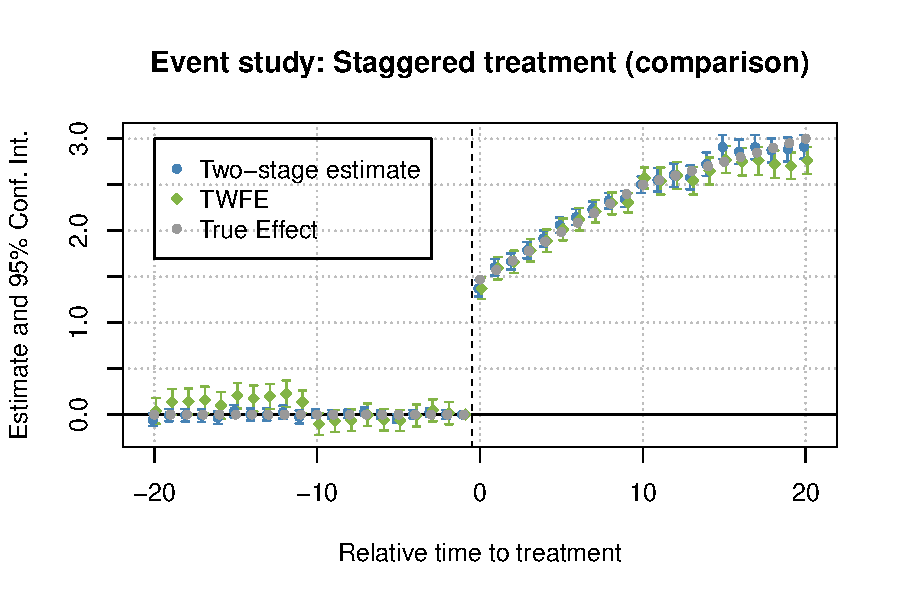
\includegraphics[width=1\linewidth]{RJ-2022-048_files/figure-latex/dynamic-w-twfe-1} \caption{This figure adds the standard ordinary-least squares estimates to the true effect and the `did2s` estimates present in Figure 2. The x-axis of this figure is the relative time to treatment, i.e. how many years pre-/post- treatment that period is. The y-axis is estimated treatment effects. There are three sets of points. The first two sets of points are the same as in Figure 2. The third set of points is the ordinary-least squares estimates. These points exhibit show evidence of parallel pre-trends failing.}\label{fig:dynamic-w-twfe}
\end{figure}

\hypertarget{the-event_study-and-plot_event_study-command}{%
\subsubsection{\texorpdfstring{The \texttt{event\_study} and \texttt{plot\_event\_study} command}{The event\_study and plot\_event\_study command}}\label{the-event_study-and-plot_event_study-command}}

The command \texttt{event\_study} presents a common syntax that estimates the event-study TWFE model for treatment-effect heterogeneity robust estimators recommended by the literature and returns all the estimates in a data.frame for easy plotting by the command \texttt{plot\_event\_study}. The general syntax is

\begin{verbatim}
event_study(
    data, yname, idname, tname, gname, 
    estimator,
    xformla = NULL, horizon = NULL, weights = NULL
)
\end{verbatim}

The option \texttt{data} specifies the data set that contains the variables for the analysis. The four other required options are all names of variables: \texttt{yname} corresponds with the outcome variable of interest; \texttt{idname} is the variable corresponding to the (unique) unit identifier, \(i\); \texttt{tname} is the variable corresponding to the time period, \(t\); and \texttt{gname} is a variable indicating the period when treatment first starts (group status).

\begin{landscape}
\begin{table}
\caption{Event Study Estimators \label{tab:estimators-latex}}
\begin{threeparttable}

\begin{tabular}{L{0.2\textwidth}L{0.2\textwidth}L{0.3\textwidth}p{0.5\textwidth}c}
\toprule
\multicolumn{1}{l}{Estimator and} & \multicolumn{1}{l}{Type} & \multicolumn{1}{l}{Comparison group} & \multicolumn{1}{c}{Main Assumptions} \\
\multicolumn{1}{l}{\texttt{R} package} & & &\\

\midrule
Gardner (2021) 
\{\texttt{did2s}\}
& Imputes $Y(0)$ 
& Not-yet- and/or Never-treated 
& 
\vspace{-5mm}
\begin{itemize}[leftmargin=*]
  \item Parallel Trends for all units
  \item Limited anticipation${^*}$
  \item Correct specification of $Y(0)$
\end{itemize}
& \\

Borusyak, Jaravel, and Spiess (2021) 
\{\texttt{didimputation}\}
& Imputes $Y(0)$ 
& Not-yet- and/or Never-treated 
& 
\vspace{-5mm}
\begin{itemize}[leftmargin=*]
  \item Parallel Trends for all units
  \item Limited anticipation${^*}$
  \item Correct specification of $Y(0)$
\end{itemize}
& \\

Callaway and Sant'Anna (2021) 
\{\texttt{did}\}
& 2$\times$2 Aggregation 
& Either Not-yet- or Never-treated 
& 
\vspace{-5mm}
\begin{itemize}[leftmargin=*]
  \item Parallel Trends for Not-yet-treated {\it or} Never-treated
  \item Limited anticipation${^*}$
\end{itemize}
& \\

Sun and Abraham (2020) 
\{\texttt{fixest}/\texttt{sunab}\}
& 2$\times$2 Aggregation 
& Not-yet- and/or Never-treated 
& 
\vspace{-5mm}
\begin{itemize}[leftmargin=*]
  \item Parallel Trends for all units
  \item Limited anticipation${^*}$
\end{itemize}
& \\

Roth and Sant'Anna (2021) 
\{\texttt{staggered}\}
& 2$\times$2 Aggregation 
& Not-yet-treated 
& 
\vspace{-5mm}
\begin{itemize}[leftmargin=*]
  \item Treatment timing is random
  \item Limited anticipation${^*}$
\end{itemize}
& \\
\bottomrule
\end{tabular}

\begin{tablenotes}
\item { This table summarizes the differences between various proposed event-study estimators in the econometric literature. It highlights the two different strategies that different estimators use, namely imputation and 2x2 aggregation. Importantly, it tries to show the differences in assumptions for each different estimator.}
\item[$^{*}$] { Anticipation can be accounted for by adjusting 'initial treatment day' back $x$ periods, where $x$ is the number of periods before treatment that anticipation can occur.}
\end{tablenotes}

\end{threeparttable}
\end{table}
\end{landscape}

There are five main estimators available and the choice is specified for the \texttt{estimator} argument and are described in Table \ref{tab:estimators-latex}.\footnote{Except for Sun and Abraham, the \texttt{estimator} option is the package name. For Sun and Abraham, the \texttt{estimator} option is \texttt{sunab}. A value of ``all'' will estimate all 5 estimators.} The following paragraphs will aim to highlight the differences and commonalities between estimators. These estimators fall into two broad categories. First, \CRANpkg{did2s} and \CRANpkg{didimputation} (Butts 2021) are \texttt{imputation-based} estimators as described above. Both rely on ``residualizing'' the outcome variable \(\tilde{Y} = Y_{it} - \hat{\mu}_g - \hat{\eta}_t\) and then averaging those \(\tilde{Y}\) to estimate the event-study average treatment effect \(\tau^k\). These two estimators return identical point estimates for post-treatment effects, but differ in their asymptotic regime and hence their standard errors.

The second type of estimator, which we label \texttt{2x2\ aggregation}, takes a different approach for estimating event-study average treatment effects. The packages \CRANpkg{did} (Callaway and Sant'Anna 2021), \CRANpkg{fixest} and \CRANpkg{staggered} (Roth and Sant'Anna 2021) first estimate \(\tau_{gt}\) for all group-time pairs. To estimate a particular \(\tau_{gt}\), they use a two-period (periods \(t\) and \(g-1\)) and two-group (group \(g\) and a ``control group'') difference-in-differences estimator, known as a \texttt{2x2} difference-in-differences. The particular ``control group'' they use will differ based on estimator and is discussed in the next paragraph. Then, the estimator manually aggregate \(\tau_{gt}\) across all groups that were treated for (at least) \(k\) periods to estimate the event-study average treatment effect \(\tau^k\).

These estimators do not all rely on the same underlying assumptions, so the rest of the table summarizes the primary differences between estimators. The comparison group column describes which units are utilized as comparison groups in the estimator and hence will determine which units need to satisfy a parallel trends assumption. For example, in some circumstances, treated units will look very different from never-treated units. In this case, parallel trends may only hold between units that receieve treatment at some point and hence only these units should be used in estimation. In other cases, for example if treatment is assigned randomly, then it's reasonable to assume that both not-yet- and never-treated units would all satisfy parallel trends.

For estimators labeled ``Not-yet- and/or never-treated'', the default is to use both not-yet- and never-treated units in the estimator. However, if all never-treated units are dropped from the data set before using the estimator, then these estimators will use only not-yet-treated groups as the comparison group. \CRANpkg{did} provides an option to use either the not-yet- treated \emph{or} the never- treated group as a comparison group depending on which group a researcher thinks will make a better comparison group. \CRANpkg{staggered} will automatically drop units that are never treated from the sample and hence only use not-yet-treated groups as a comparison group.

The next column, \texttt{Main\ Assumptions}, summarize concisely the main theoretical assumptions underlying each estimator. First, the assumptions about parallel trends match the previous discussion on the correct comparison group. The only estimator that doesn't rely on a parallel trends assumption is \CRANpkg{staggered} which relies on the assumption that \emph{when} a unit receives treatment is random.

The next assumption, that is common across all estimators, is that there should be ``limited anticipation'' of treatment. In general, anticipatory effects are when units respond to treatment before it is \emph{actually} implemented. For example, this can be common if the news of a policy triggers behavior responses before the treatment is put in place. ``Limited anticipation'' is when these anticipatory effects can only exist in a ``few'' pre-periods.\footnote{There should be more periods before treatment in the sample than whatever number a ``few'' is.} In any of these cases, ``treatment'' should be manually moved back by the maximum number of periods where anticipation can occur. For example, if treatment starts in 2012 and anticipatory effects are reasonably only possible 2 years before, this units' ``group'' should be labeled as 2010 in the data.

The \texttt{imputation-based} estimators require an additional assumption that the parametric model of \(Y(0) = \mu_i + \eta_t + \varepsilon_{it}\) is correctly specified. This is because in the first stage, you have to accurately impute \(Y(0)\) when residualizing \(Y\) which relies on the correct specification of \(Y(0)\). The \texttt{2x2\ aggregation} models do not estimate a parametric form of \(Y(0)\) and hence only relies on a parallel trends assumption. While not in the table, it is worth noting that \CRANpkg{did} allows for uniform inference of estimates. This addresses the problem that multiple hypotheses tests are being done by researchers (e.g.~checking individually if all post period estimates are significant) by creating standard errors that adjust for multiple testing.

\hypertarget{example-usage-of-event_study}{%
\paragraph{\texorpdfstring{Example usage of \texttt{event\_study}}{Example usage of event\_study}}\label{example-usage-of-event_study}}

The result of \texttt{event\_study} is a tibble in a \texttt{tidy} format (Robinson, Hayes, and Couch 2021) that contains point estimates and standard errors for each relative time indicator for each estimator. The results of \texttt{event\_study} are stored as a dataframe with event-study term, the estimate, standard error, and a column containing which estimator is used for that estimate. This output dataframe will in turn be passed to \texttt{plot\_event\_study} for easy comparison. \texttt{plot\_event\_study} will return a \texttt{ggplot} object (Wickham 2016). We return to the \texttt{df\_het} dataset to see example usage of these functions.

\begin{verbatim}
data(df_het, package = "did2s")
out = event_study(
  data = df_het, yname = "dep_var", idname = "unit",
  tname = "year", gname = "g", estimator = "all"
)
\end{verbatim}

\begin{verbatim}
head(out)
\end{verbatim}

\begin{verbatim}
#>    estimator term   estimate  std.error
#> 1:      TWFE  -20 0.04097725 0.07167704
#> 2:      TWFE  -19 0.13665695 0.07147683
#> 3:      TWFE  -18 0.14015820 0.07245520
#> 4:      TWFE  -17 0.15793252 0.07431871
#> 5:      TWFE  -16 0.09910002 0.07379570
#> 6:      TWFE  -15 0.20561127 0.07116478
\end{verbatim}

\begin{verbatim}
plot_event_study(out, horizon = c(-5, 10))
\end{verbatim}

\begin{figure}
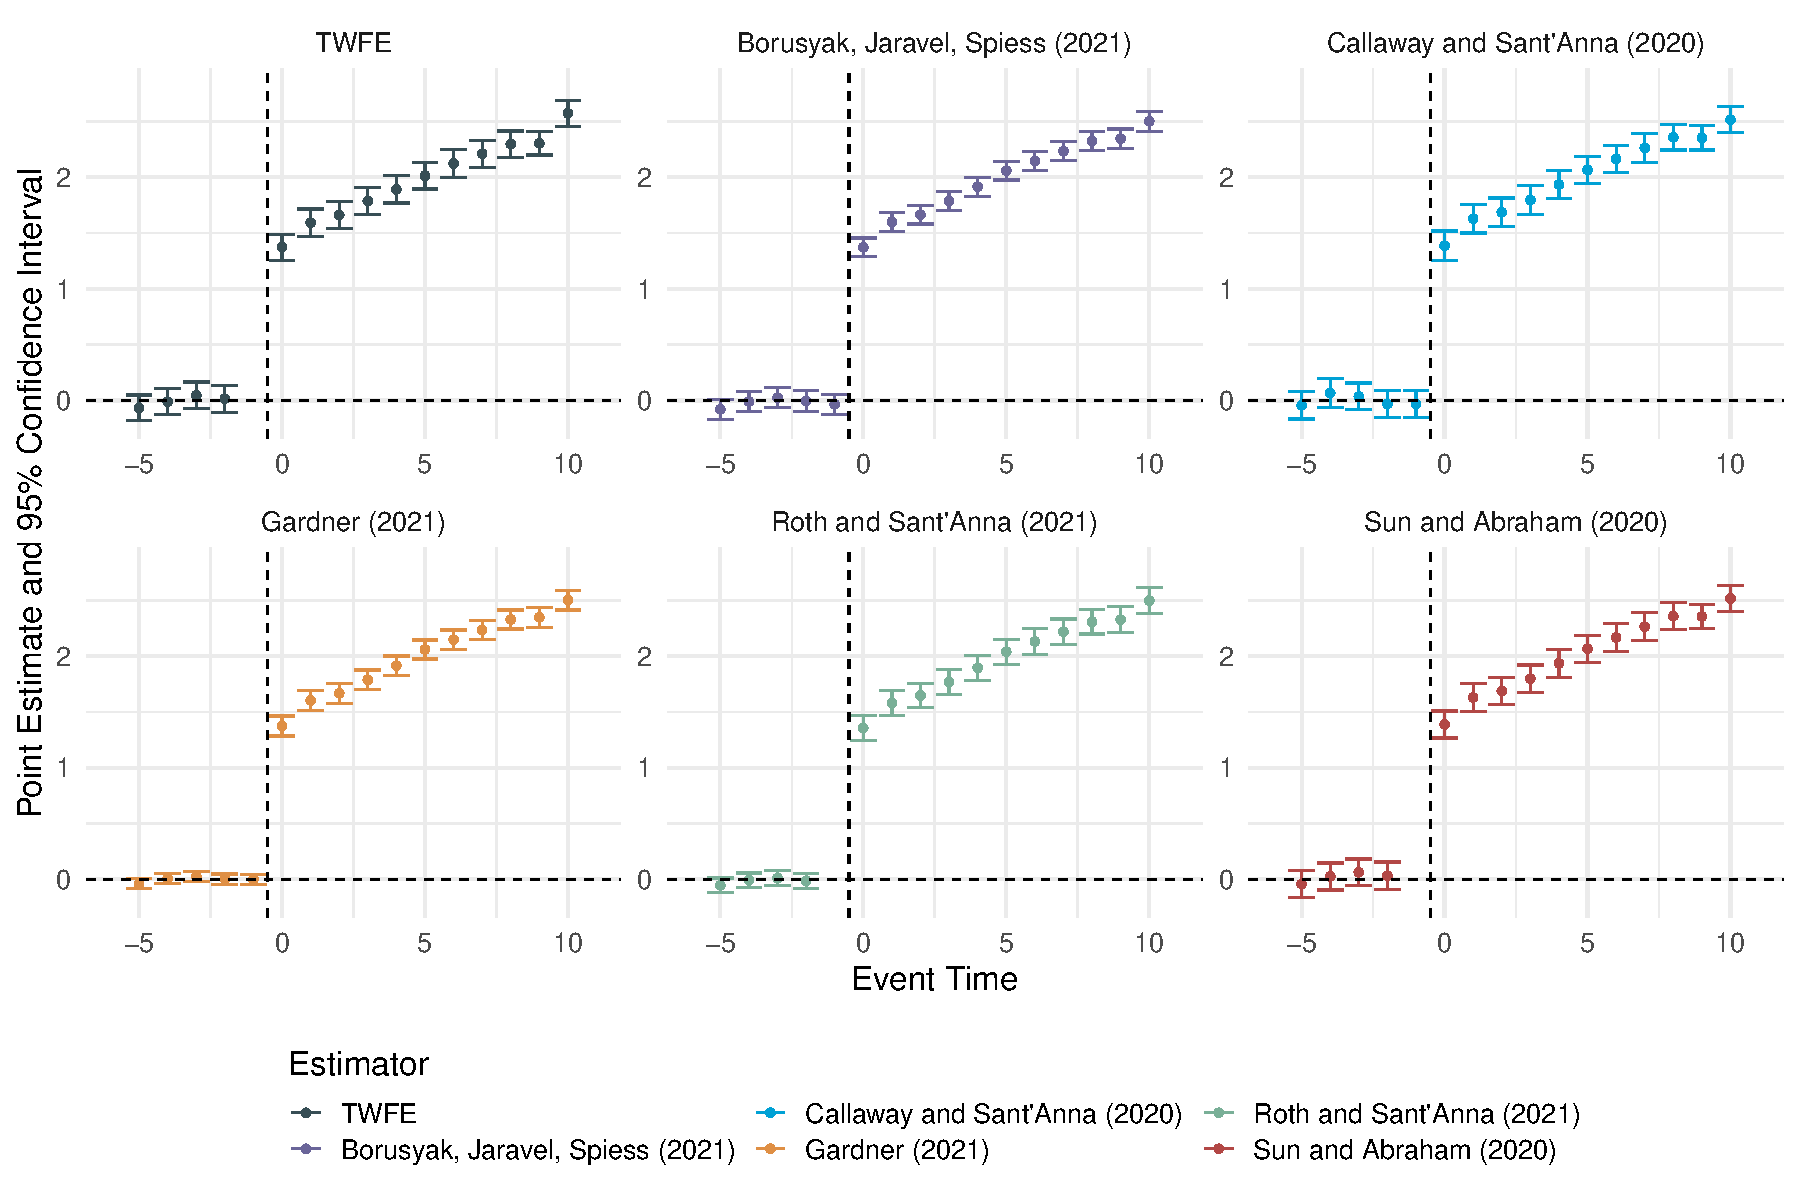
\includegraphics[width=1\linewidth]{RJ-2022-048_files/figure-latex/es-alternatives-1} \caption{This figure contains six plots displayed in a grid of different event study estimators. The estimators are labeled 'TWFE', 'Borusyak, Jaravel, Spiess (2021)', 'Callaway and Sant'Anna (2020)', 'Gardner (2021)', 'Roth and Sant'Anna (2021)', and 'Sun and Abraham (2020)'. Each estimator's necessary assumptions are described above. Each plot in the figure displays point estimates from pre-treatment year -5 through post-treatment year 10. Each estimator is approximately 0 for all pre-treatment periods. In post-periods, each figure follows the true treatment effect starting at 1.5 in post-period 1 and growing afterwards.}\label{fig:es-alternatives}
\end{figure}

\hypertarget{conclusion}{%
\subsection{Conclusion}\label{conclusion}}

This article introduced the package \CRANpkg{did2s} which provides a fast, memory-efficient, and treatment-effect heterogeneity robust way to estimate two-way fixed-effect models. The package also includes the \texttt{event\_study} and \texttt{plot\_event\_study} functions to allow for a single syntax for the various estimators introduced in the literature. A companion package in Stata is also available with similar syntax for the \texttt{did2s} function.

While this package includes an event\_study function that aims to help individuals implement any of the proposed modern ``solutions'' to the difference-in-differences estimation, further research on this topic is needed to help practitioners be able to more precisely determine which estimators work best in their settings. Potentially, there could be data-driven methods to try to identify the plausibility of the different assumptions. Additionally, there is still more work to be done to formalize under what conditions covariates can flexibly be used in estimation. There is some initial work from Caetano et al. (2022), but there does not yet exist statistical software to perform their proposed estimator.

\hypertarget{references}{%
\section*{References}\label{references}}
\addcontentsline{toc}{section}{References}

\hypertarget{refs}{}
\begin{CSLReferences}{1}{0}
\leavevmode\vadjust pre{\hypertarget{ref-Berge_2018}{}}%
Bergé, Laurent. 2018. {``Efficient Estimation of Maximum Likelihood Models with Multiple Fixed-Effects: The {R} Package {FENmlm}.''} \emph{CREA Discussion Papers}, no. 13.

\leavevmode\vadjust pre{\hypertarget{ref-Borusyak_Jaravel_Spiess_2021}{}}%
Borusyak, Kirill, Xavier Jaravel, and Jann Spiess. 2021. {``Revisiting Event Study Designs: Robust and Efficient Estimation.''} Working Paper.

\leavevmode\vadjust pre{\hypertarget{ref-didimputation}{}}%
Butts, Kyle. 2021. \emph{Didimputation: Difference-in-Differences Estimator from Borusyak, Jaravel, and Spiess (2021)}. \url{https://www.github.com/kylebutts/didimputation}.

\leavevmode\vadjust pre{\hypertarget{ref-Caetano_Callaway_Payne_Rodrigues_2022}{}}%
Caetano, Carolina, Brantly Callaway, Stroud Payne, and Hugo Sant'Anna Rodrigues. 2022. {``Difference in Differences with Time-Varying Covariates.''} Working Paper. \url{http://arxiv.org/abs/2202.02903}.

\leavevmode\vadjust pre{\hypertarget{ref-Callaway_SantAnna_2020}{}}%
Callaway, Brantly, and Pedro H. C. Sant'Anna. 2020. {``Difference-in-Differences with Multiple Time Periods.''} \emph{Journal of Econometrics}. https://doi.org/\url{https://doi.org/10.1016/j.jeconom.2020.12.001}.

\leavevmode\vadjust pre{\hypertarget{ref-did}{}}%
---------. 2021. \emph{Did: Difference in Differences}. \url{https://bcallaway11.github.io/did/}.

\leavevmode\vadjust pre{\hypertarget{ref-deChaisemartin_DHaultfoeuille_2019}{}}%
Chaisemartin, Clément de, and Xavier D'Haultfoeuille. 2019. \emph{Two-Way Fixed Effects Estimators with Heterogeneous Treatment Effects}. w25904. National Bureau of Economic Research. \url{https://doi.org/10.3386/w25904}.

\leavevmode\vadjust pre{\hypertarget{ref-Frisch_Waugh_1933}{}}%
Frisch, Ragnar, and Frederick V. Waugh. 1933. {``Partial Time Regressions as Compared with Individual Trends.''} \emph{Econometrica} 1 (4): 387--401. \url{http://www.jstor.org/stable/1907330}.

\leavevmode\vadjust pre{\hypertarget{ref-Gardner_2021}{}}%
Gardner, John. 2022. {``Two-Stage Differences in Differences.''} arXiv. \url{https://doi.org/10.48550/ARXIV.2207.05943}.

\leavevmode\vadjust pre{\hypertarget{ref-Goodman-Bacon_2018}{}}%
Goodman-Bacon, Andrew. 2018. \emph{Difference-in-Differences with Variation in Treatment Timing}. w25018. National Bureau of Economic Research. \url{https://doi.org/10.3386/w25018}.

\leavevmode\vadjust pre{\hypertarget{ref-newey_mcfadden_1994}{}}%
Newey, Whitney, and Daniel McFadden. 1986. {``Large Sample Estimation and Hypothesis Testing.''} In \emph{Handbook of Econometrics}, edited by R. F. Engle and D. McFadden, 1st ed., 4:2111--2245. Elsevier. \url{https://EconPapers.repec.org/RePEc:eee:ecochp:4-36}.

\leavevmode\vadjust pre{\hypertarget{ref-broom}{}}%
Robinson, David, Alex Hayes, and Simon Couch. 2021. \emph{Broom: Convert Statistical Objects into Tidy Tibbles}. \url{https://CRAN.R-project.org/package=broom}.

\leavevmode\vadjust pre{\hypertarget{ref-staggered}{}}%
Roth, Jonathan, and Pedro H. C. Sant'Anna. 2021. \emph{Staggered: Efficient Estimation Under Staggered Treatment Timing}. \url{https://github.com/jonathandroth/staggered}.

\leavevmode\vadjust pre{\hypertarget{ref-Sun_Abraham_2020}{}}%
Sun, Liyang, and Sarah Abraham. 2020. {``Estimating Dynamic Treatment Effects in Event Studies with Heterogeneous Treatment Effects.''} \emph{Journal of Econometrics}, December. \url{https://doi.org/10.1016/j.jeconom.2020.09.006}.

\leavevmode\vadjust pre{\hypertarget{ref-ggplot2}{}}%
Wickham, Hadley. 2016. \emph{Ggplot2: Elegant Graphics for Data Analysis}. Springer-Verlag New York. \url{https://ggplot2.tidyverse.org}.

\end{CSLReferences}

\bibliography{did2s.bib}

\address{%
Kyle Butts\\
University of Colorado Boulder\\%
\\
%
\url{https://www.kylebutts.com/}\\%
\textit{ORCiD: \href{https://orcid.org/0000-0002-9048-8059}{0000-0002-9048-8059}}\\%
\href{mailto:buttskyle96@gmail.com}{\nolinkurl{buttskyle96@gmail.com}}%
}

\address{%
John Gardner\\
University of Mississippi\\%
\\
%
\url{https://jrgcmu.github.io/}\\%
%
\href{mailto:jrgardne@olemiss.edu}{\nolinkurl{jrgardne@olemiss.edu}}%
}
